\subsection{测试用例一}
\begin{enumerate}[label = \alph*)]
  \item 测试用例描述:

  基本功能
  \item 测试目的:

  测试智能插座连接一个手机的功能
  \item 操作过程及其结果:

  通过手机热点组网进行连接,观察app指示灯的状态以及测试基本功能,发现可以手机可以发送命令
  控制插座的连接状态,也可以测量电压电流值等,基本功能完好,如图(\ref{正常工作})所示。
  通过app读取数据在表(\ref{数据})。
  \begin{table}[htbp]
    \centering
    \caption{用程序读取到的数据}
    \label{数据}
    \begin{tabular}{L{.1\textwidth}C{.15\textwidth}C{.15\textwidth}C{.15\textwidth}C{.15\textwidth}}
      \toprule
      项目  & 温度  & 电流值  & 电压值  & 功率  \\
      \midrule
      台灯 & 30.8\textcelsius & 0.17A & 4.87V & 0.87W \\
      风扇一档 & 30.9\textcelsius & 0.21A & 4.58V & 1.11W \\
      风扇二档 & 30.9\textcelsius & 0.32A & 4.72V & 1.49W \\
      \bottomrule
    \end{tabular}
  \end{table}
  \begin{figure}[htbp]
    \centering
    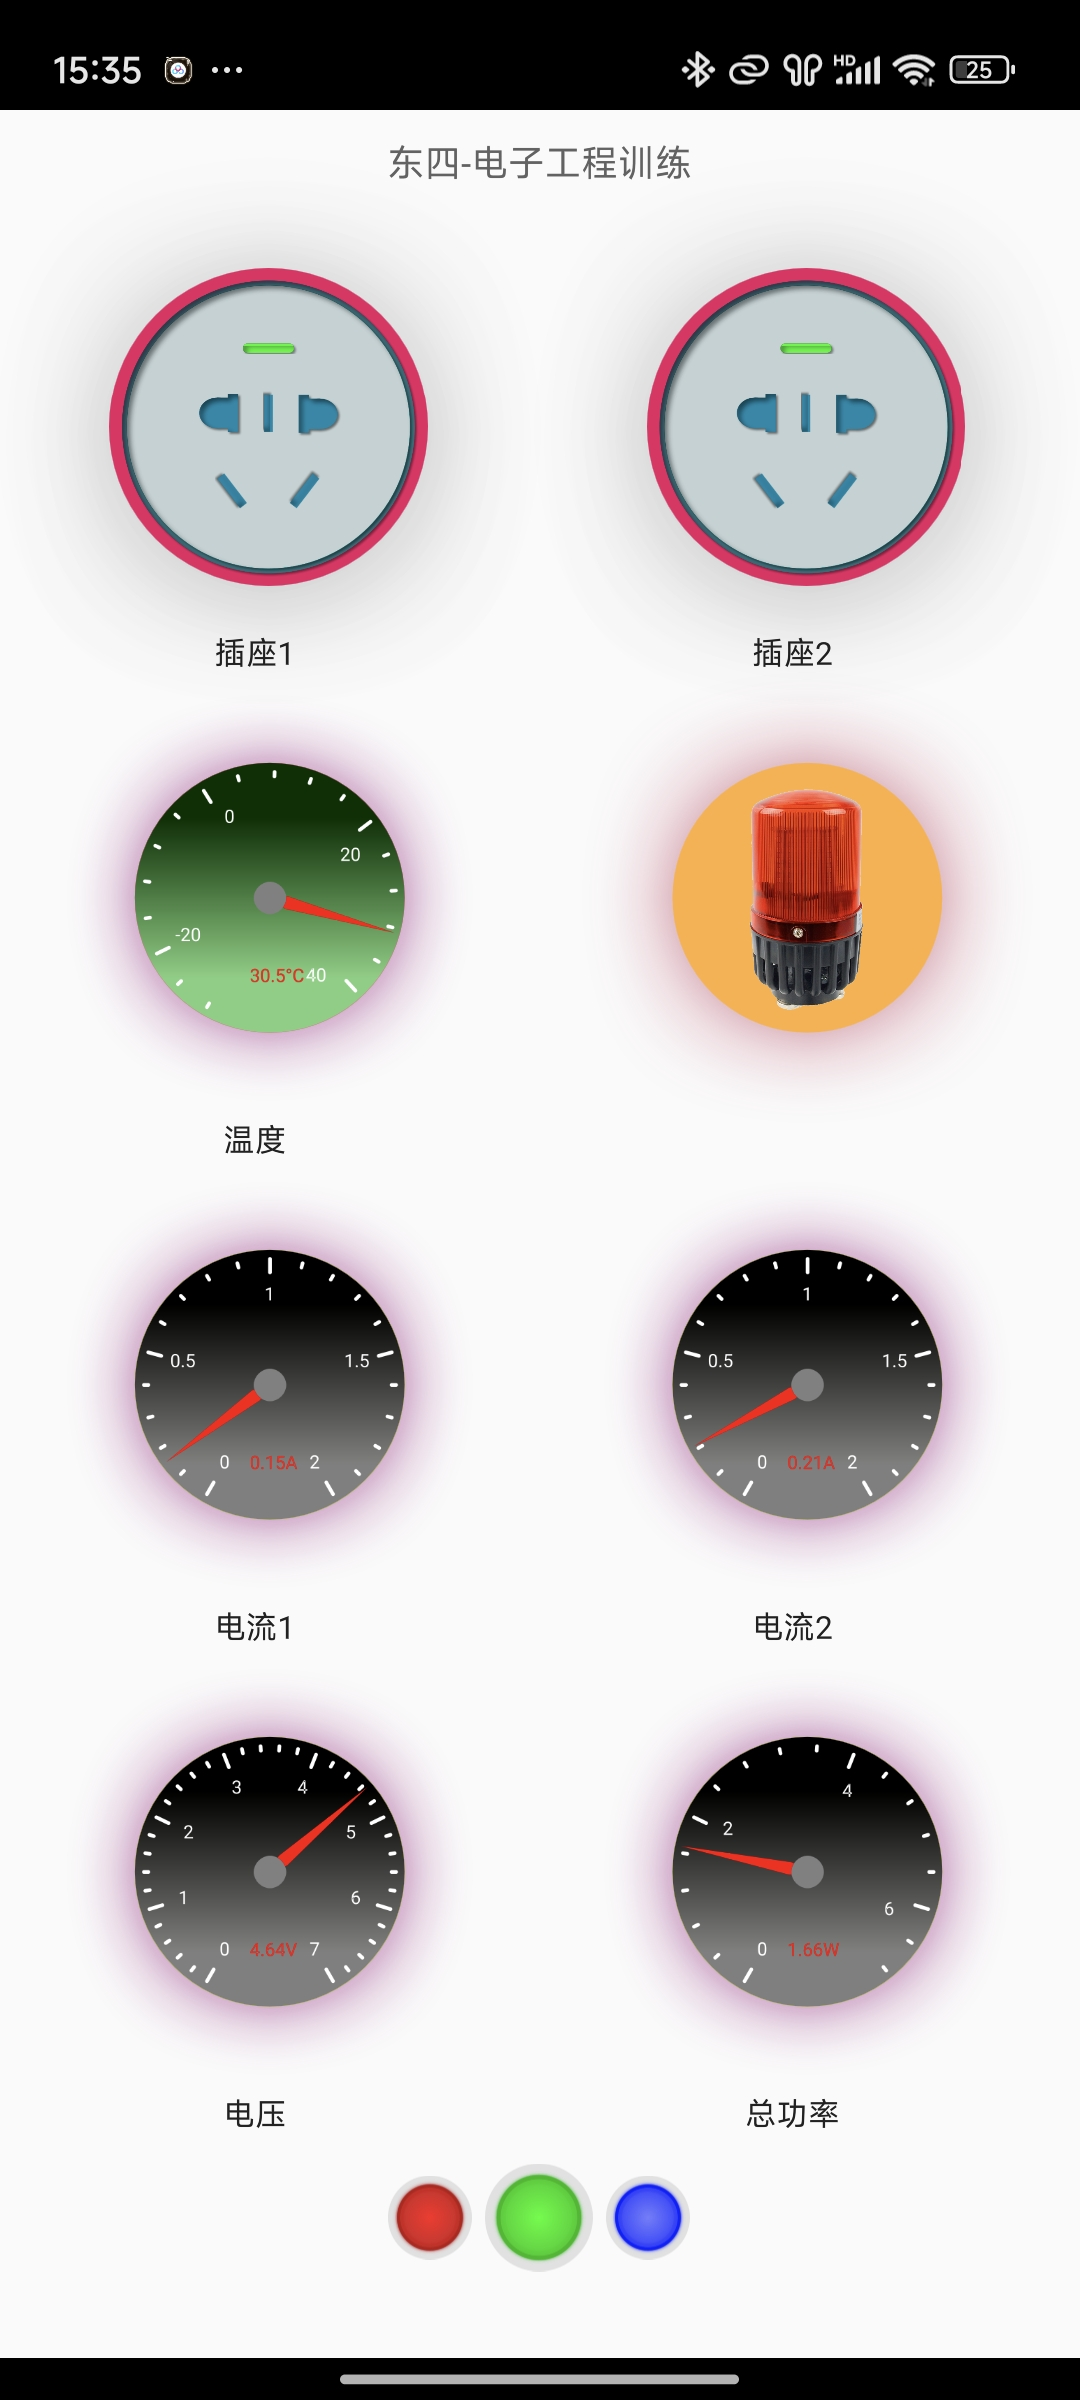
\includegraphics[width=.3\textwidth]{./figures/插座/系统调试/连接.jpg}
    \caption{正常工作}
    \label{正常工作}
  \end{figure}
\end{enumerate}
\subsection{测试用例二}
\begin{enumerate}[label = \alph*)]
  \item 测试用例描述:

  定时开关,延时开关
  \item 测试目的:

  智能插座具备定时开/关、延时开/关的功能
  \item 操作过程及其结果:

  通过设置插座定时,延时,观察开关是否在时间到的时候相应,发现功能完好,如图(\ref{定时})所示。
  \begin{figure}[htbp]
    \centering
    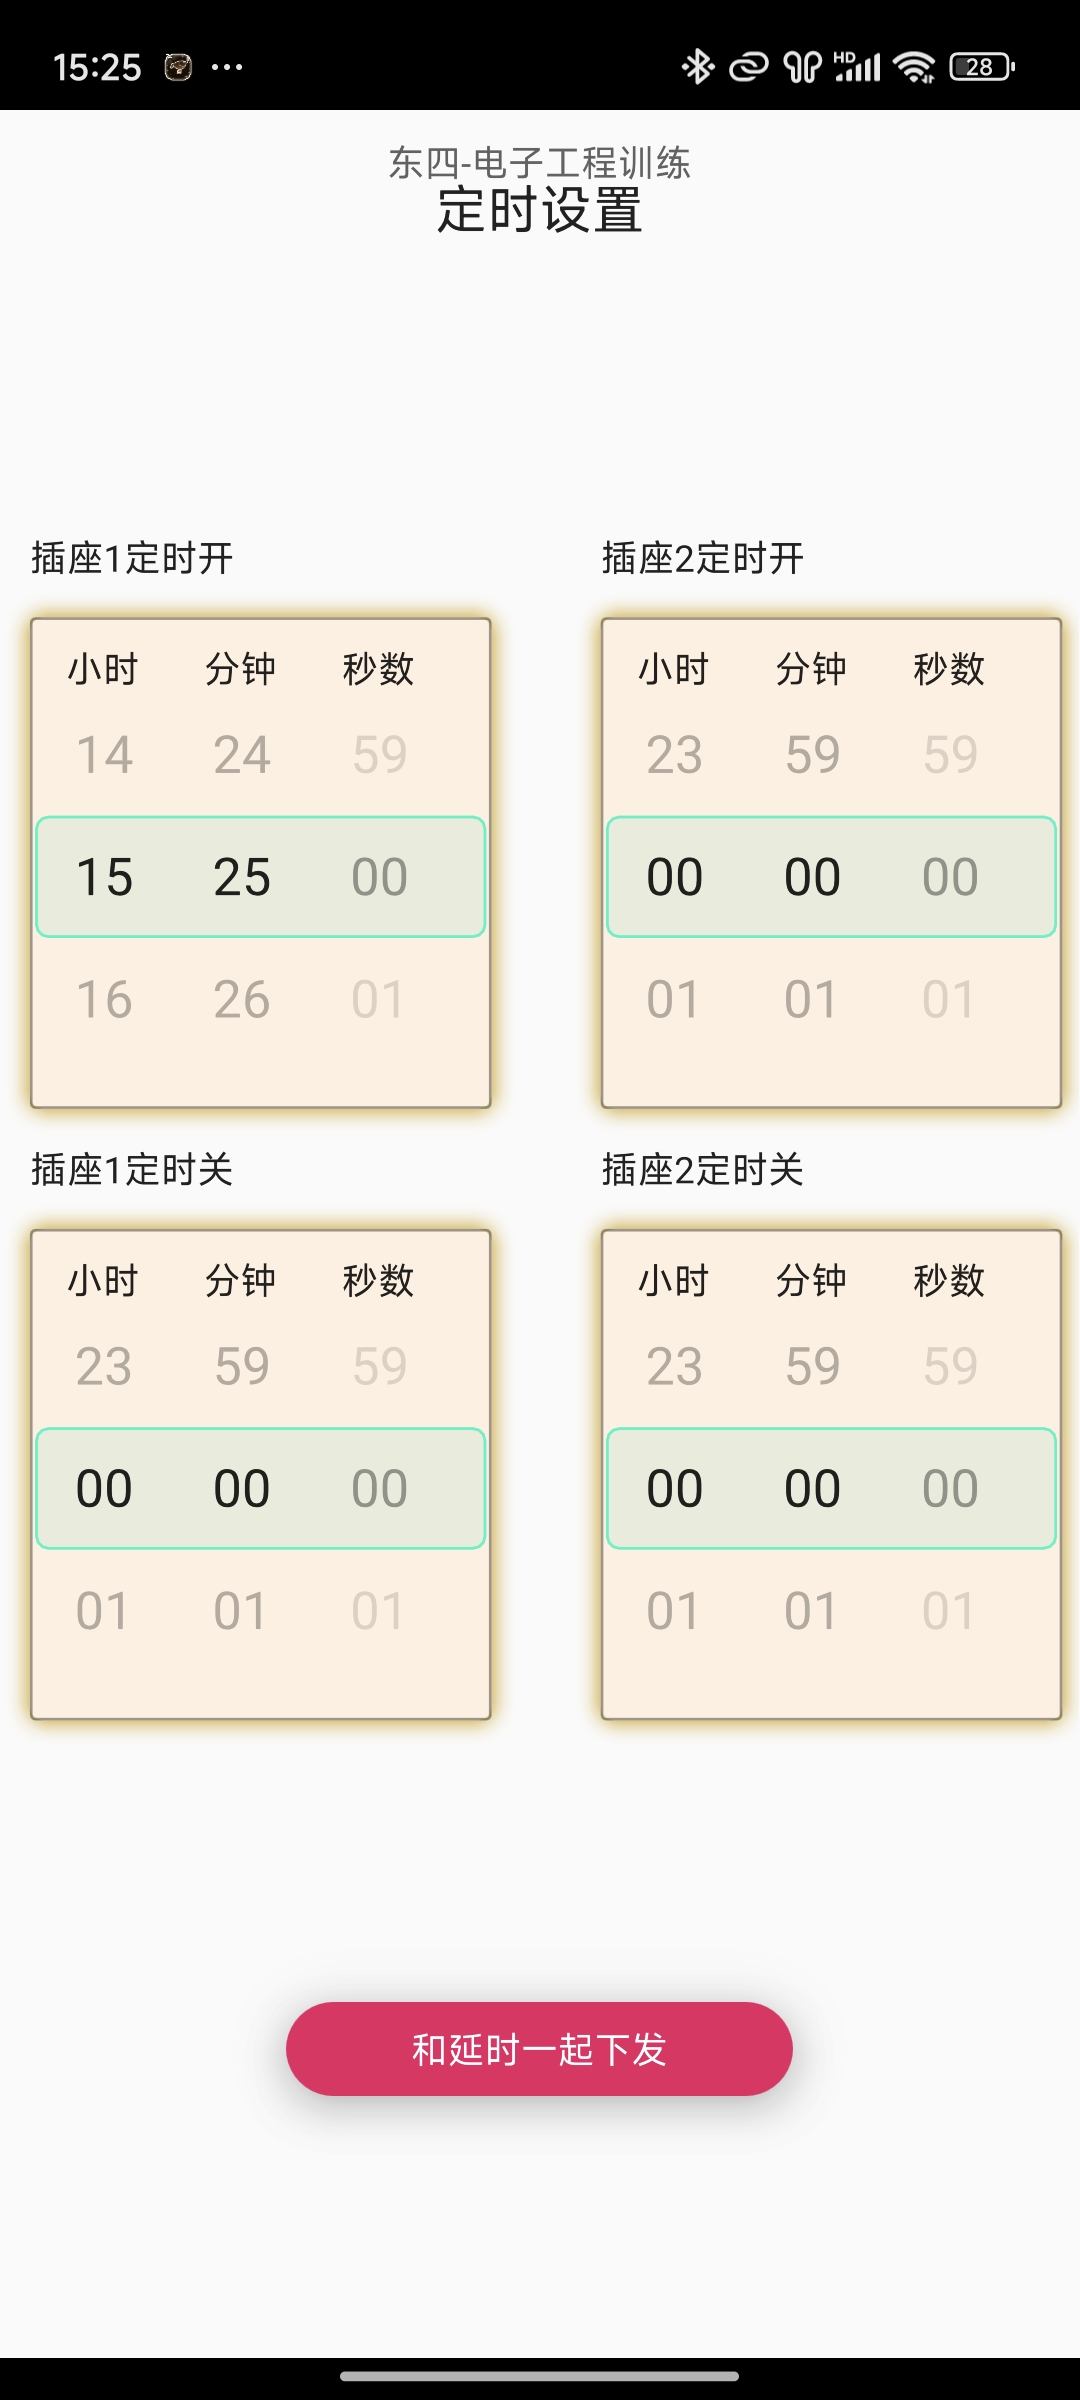
\includegraphics[width=.3\textwidth]{./figures/插座/系统调试/定时.jpg}
    \hspace{5em}
    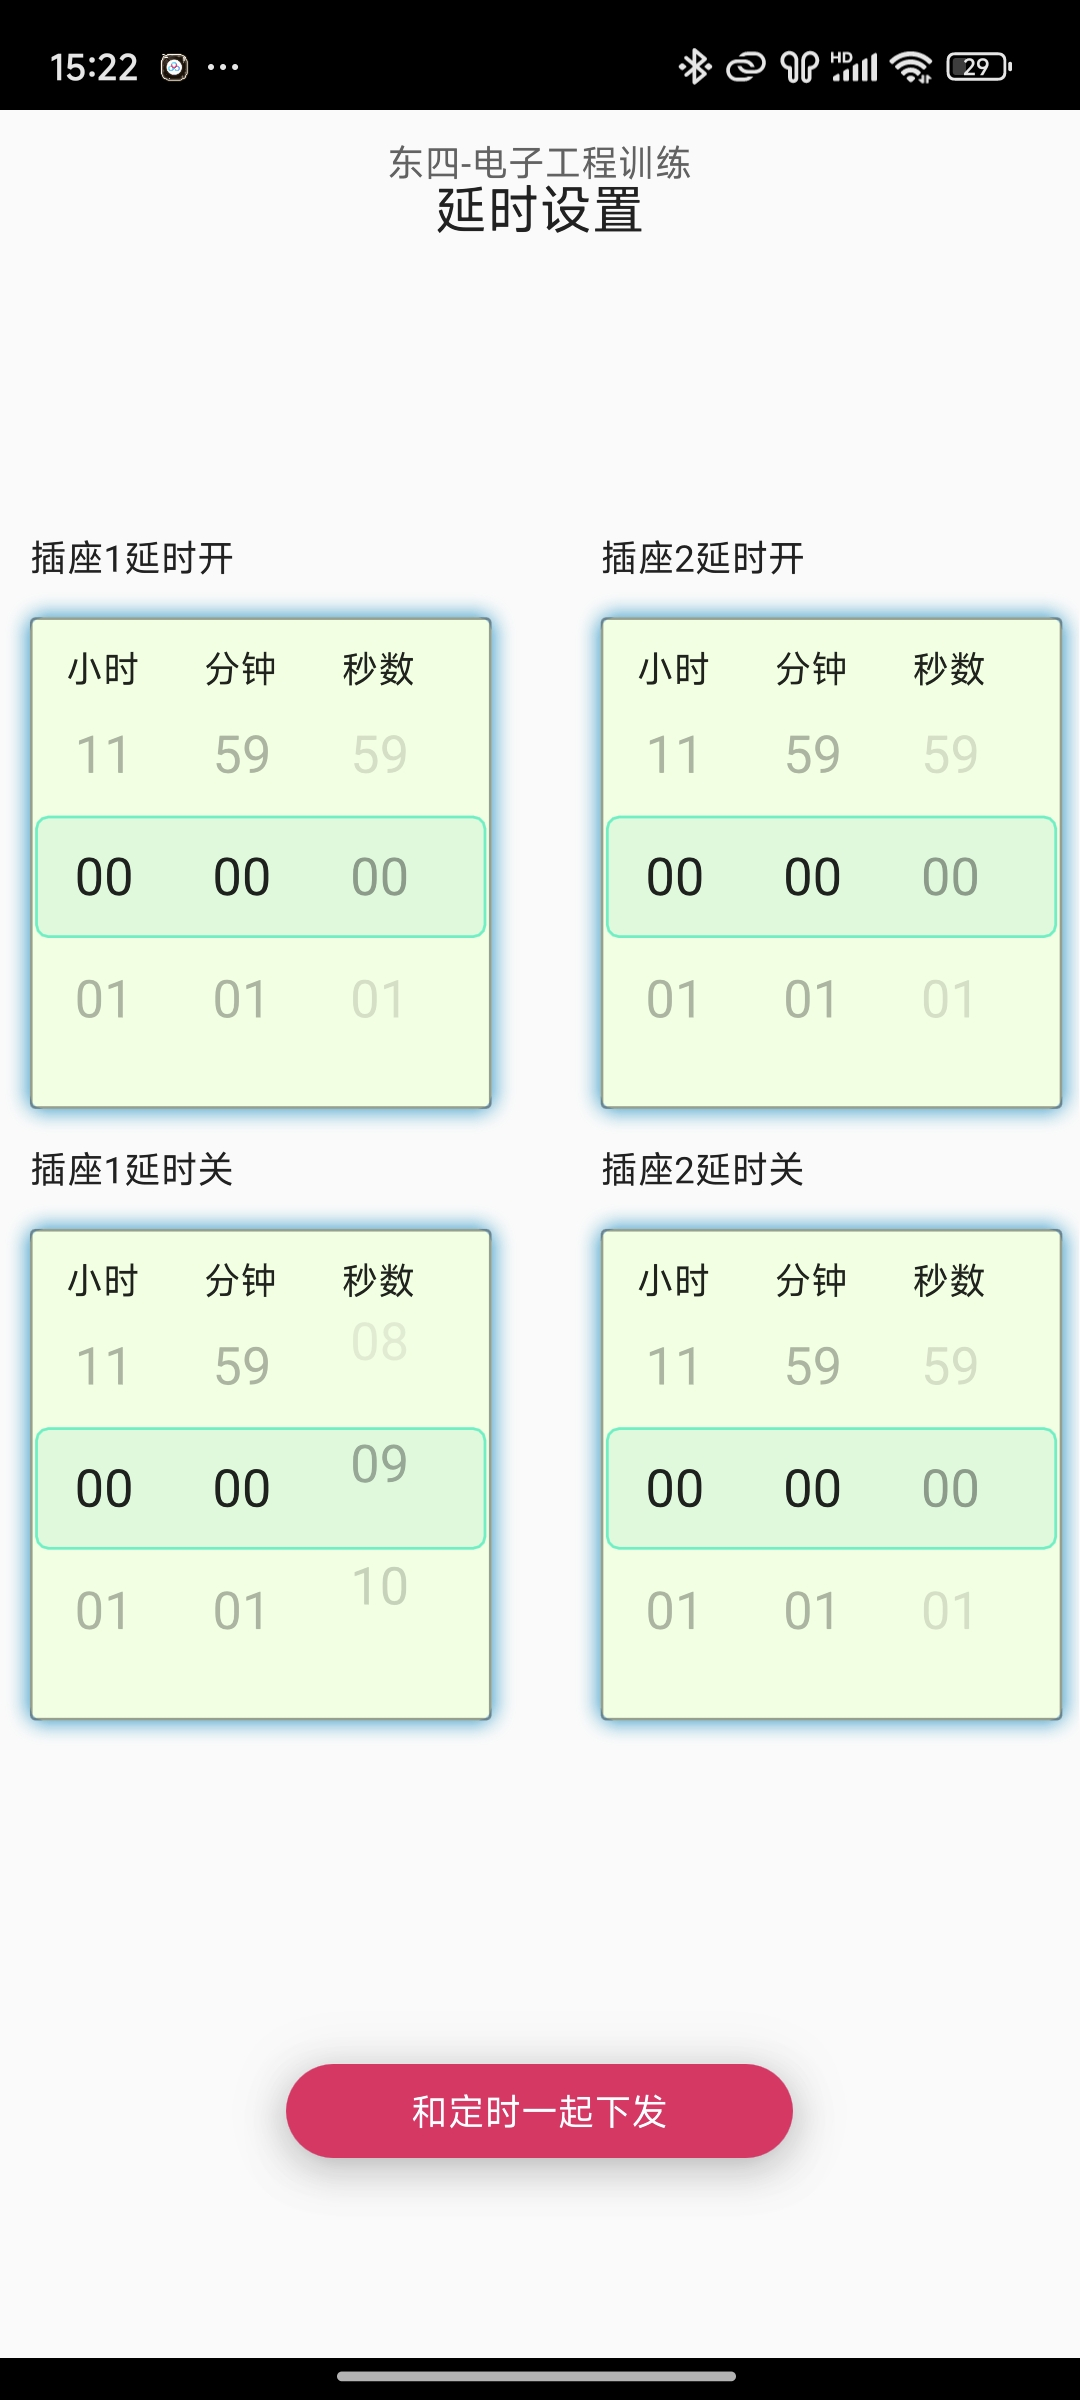
\includegraphics[width=.3\textwidth]{./figures/插座/系统调试/延时.jpg}
    \caption{插座设置定时,延时启动}
    \label{定时}
  \end{figure}
\end{enumerate}
\subsection{测试用例三}
\begin{enumerate}[label = \alph*)]
  \item 测试用例描述:

  针对超/欠电压、超电流、超功率告警并自动断开插座供电。
  \item 测试目的:

  测试插座的告警功能。
  \item 操作过程及其结果:
  \begin{enumerate}
    \item 测试子项目:超/欠电压

    测试过程:先保持下限设为最低,电压上限设为4.6V,打开插座后立即告警,恢复后将电压下限设为4.2V,上限最高
    并按下SW1使电压下降,发现插座立刻告警并断开供电。如图(\ref{电压})所示。

    \begin{figure}[htbp]
        \centering
        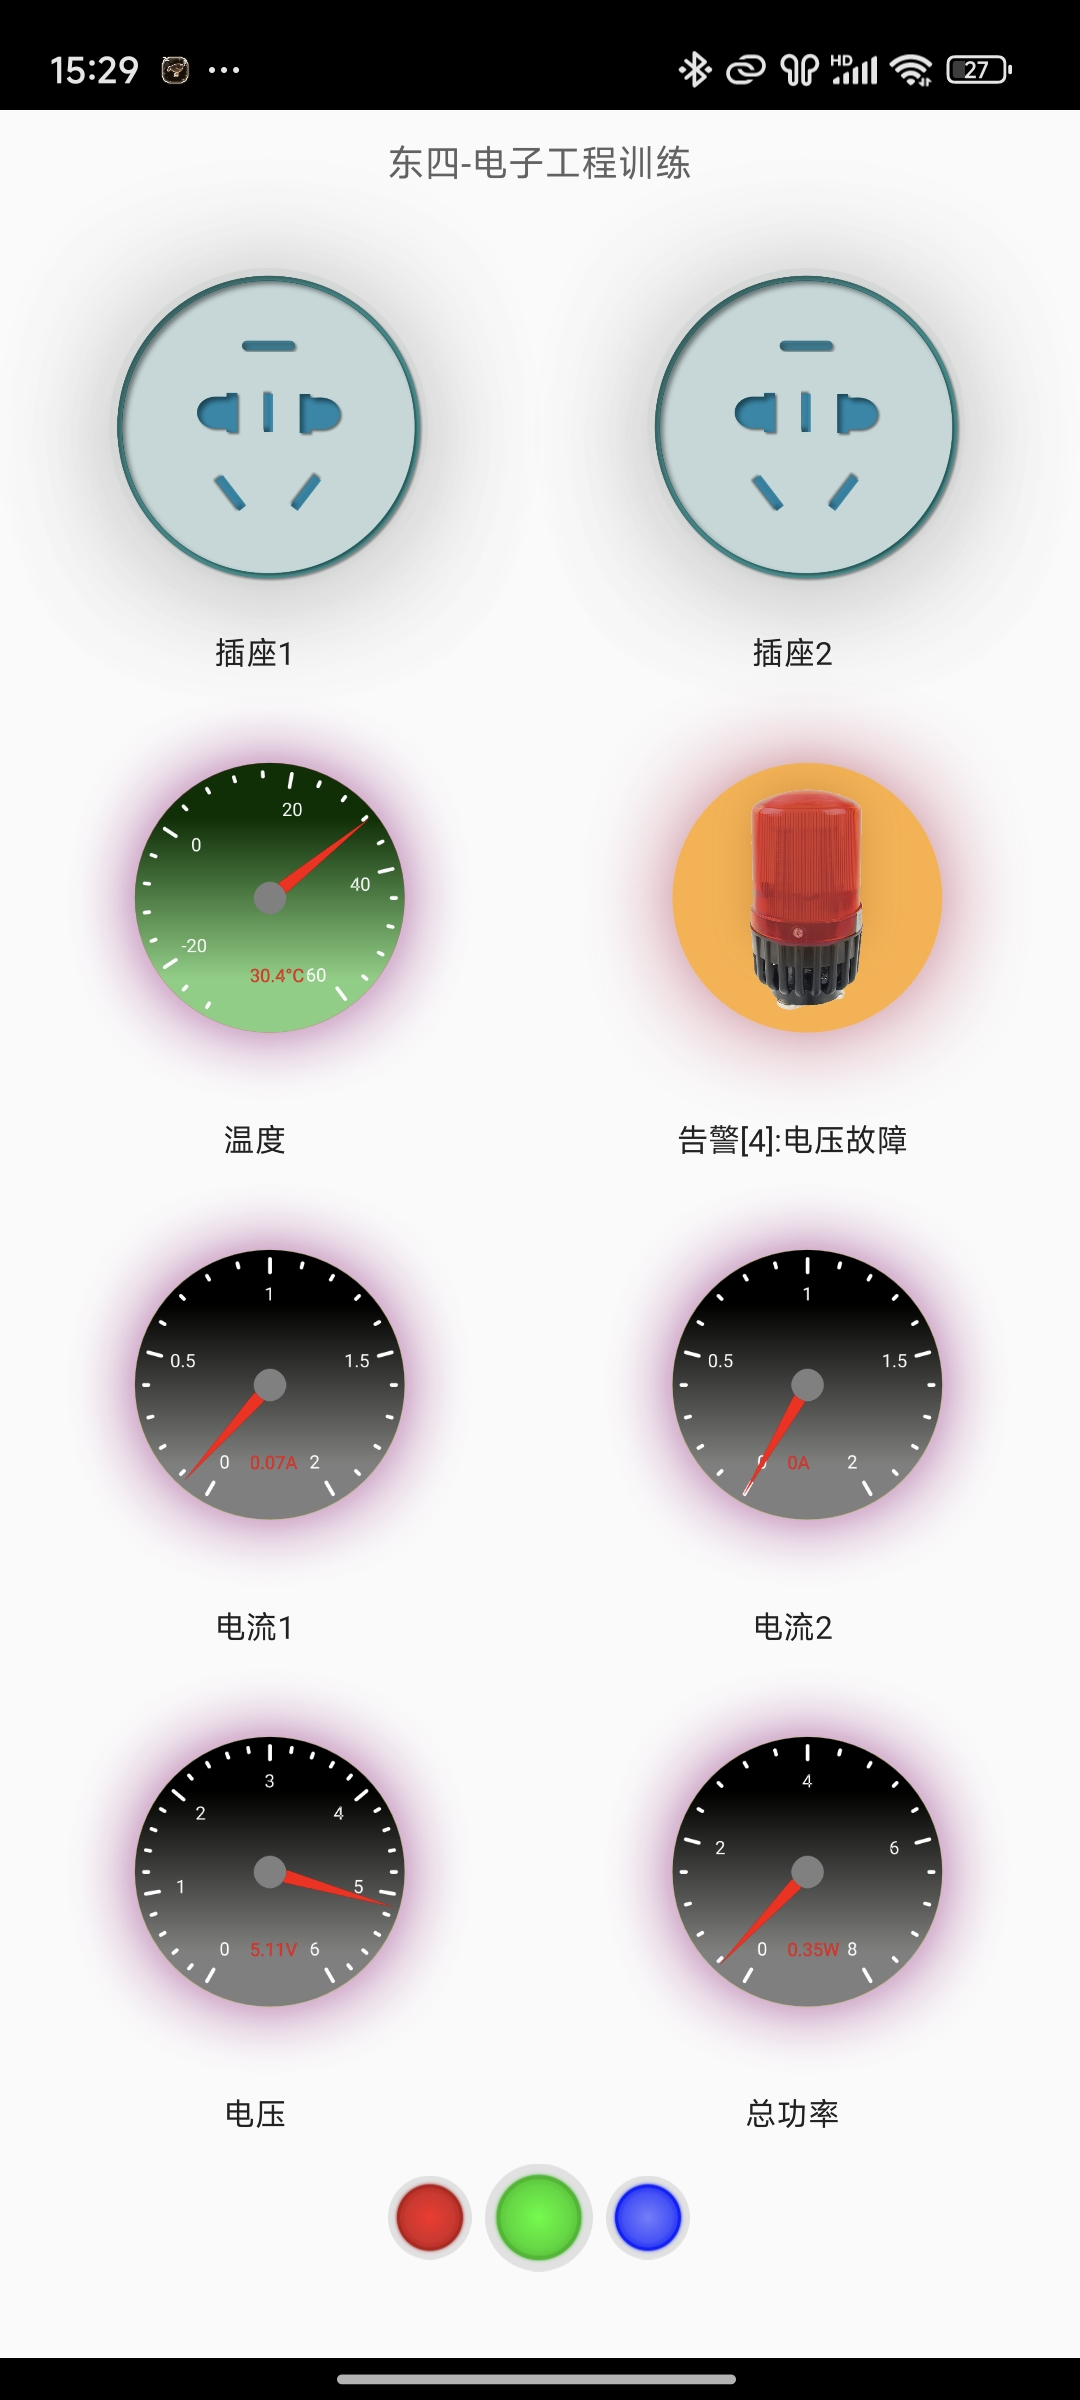
\includegraphics[width=.3\textwidth]{./figures/插座/系统调试/电压超限.jpg}
        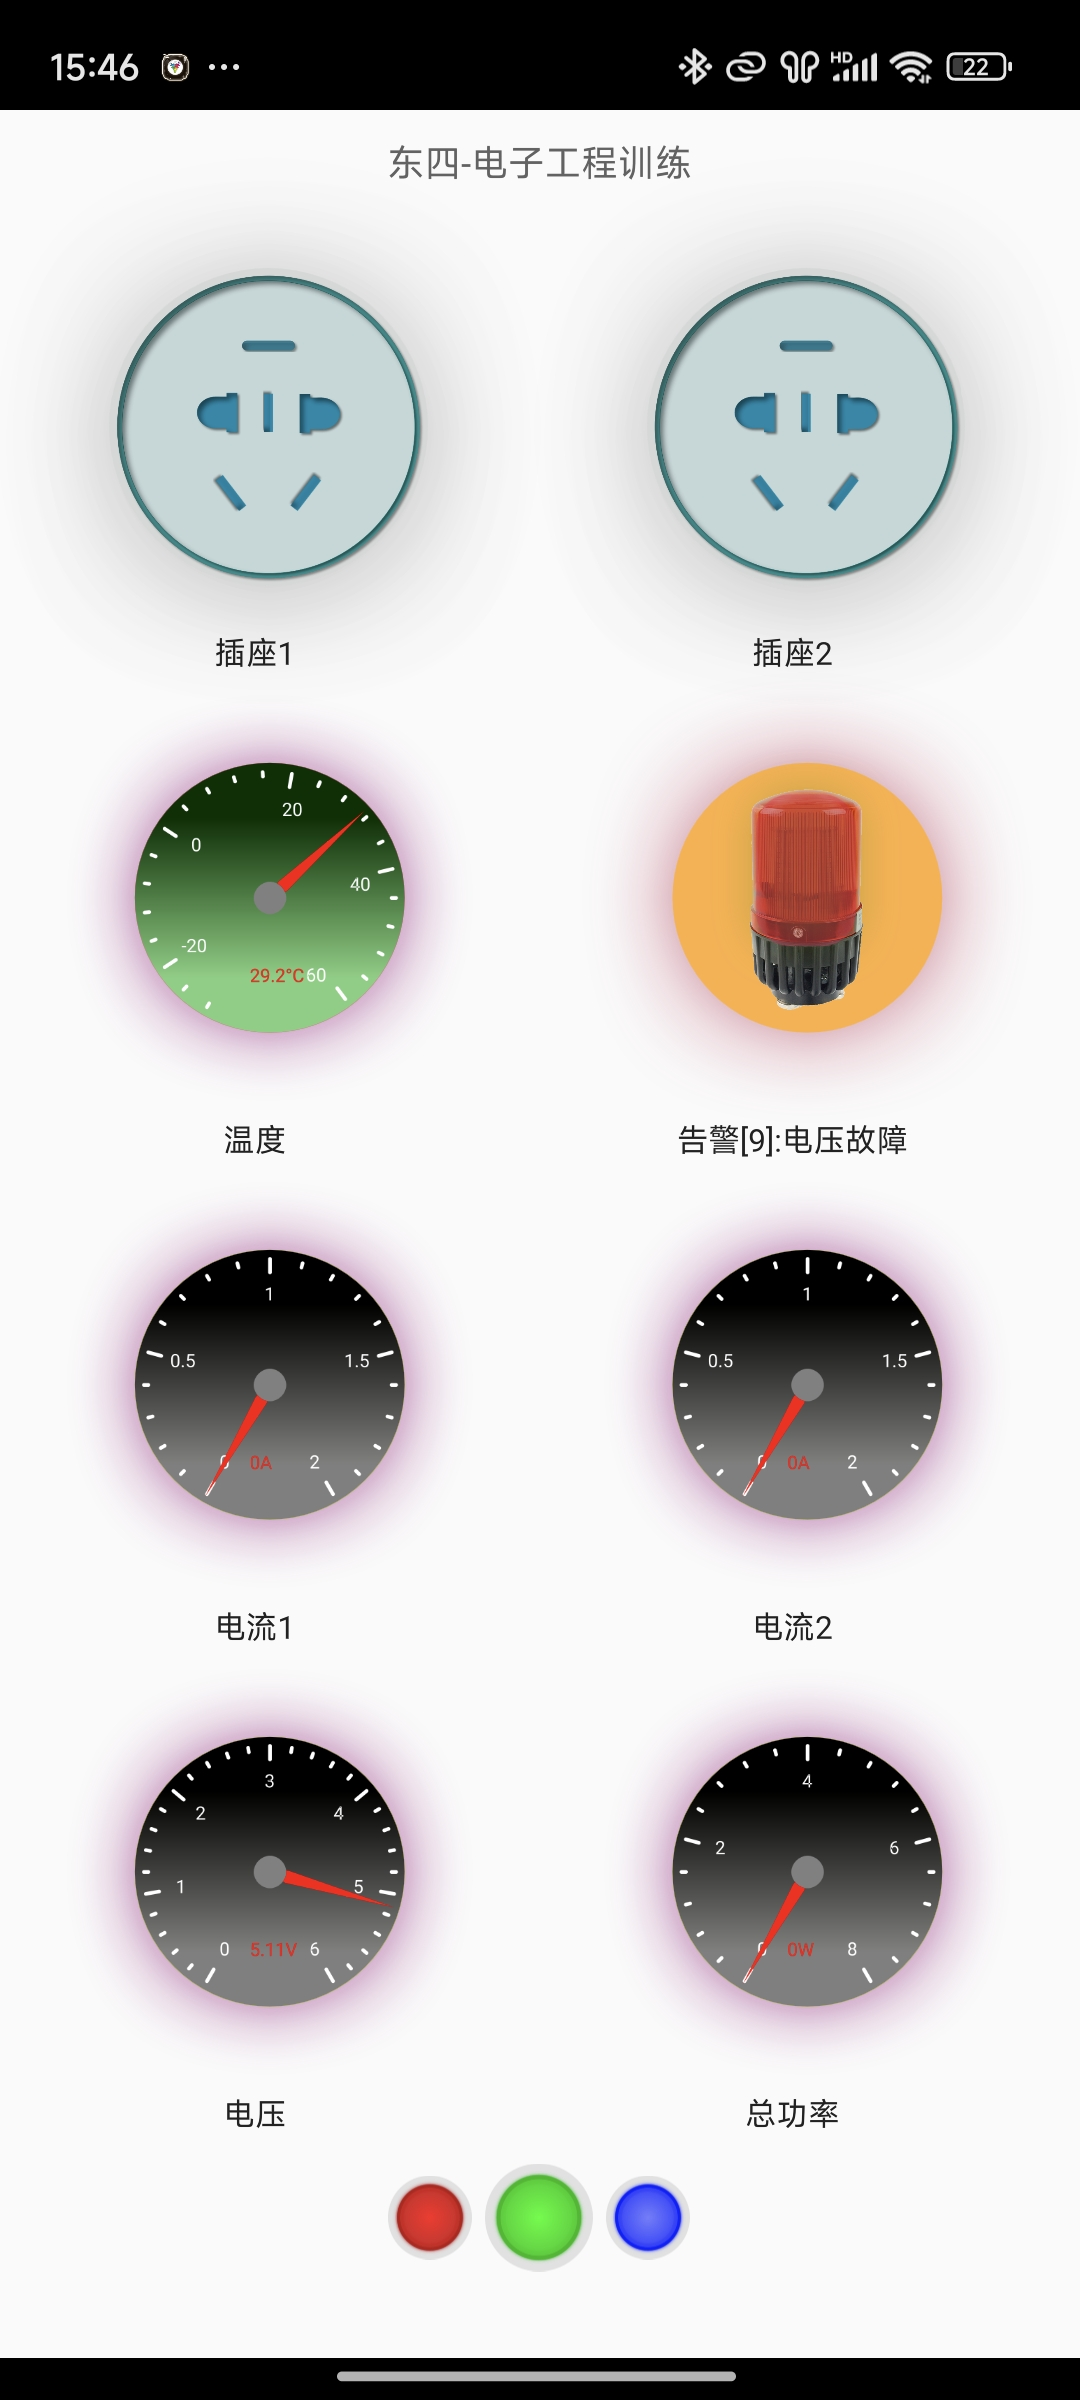
\includegraphics[width=.3\textwidth]{./figures/插座/系统调试/电压过低.jpg}
        \caption{插座关于电压的告警}
        \label{电压}
      \end{figure}

    \item 测试子项目:超电流

    测试过程:设置电流上限为0.1A,接入小风扇并调至三档,立刻给出电流超限告警并断开了插座供电,如图(\ref{电流})所示。

    \begin{figure}[htbp]
        \centering
        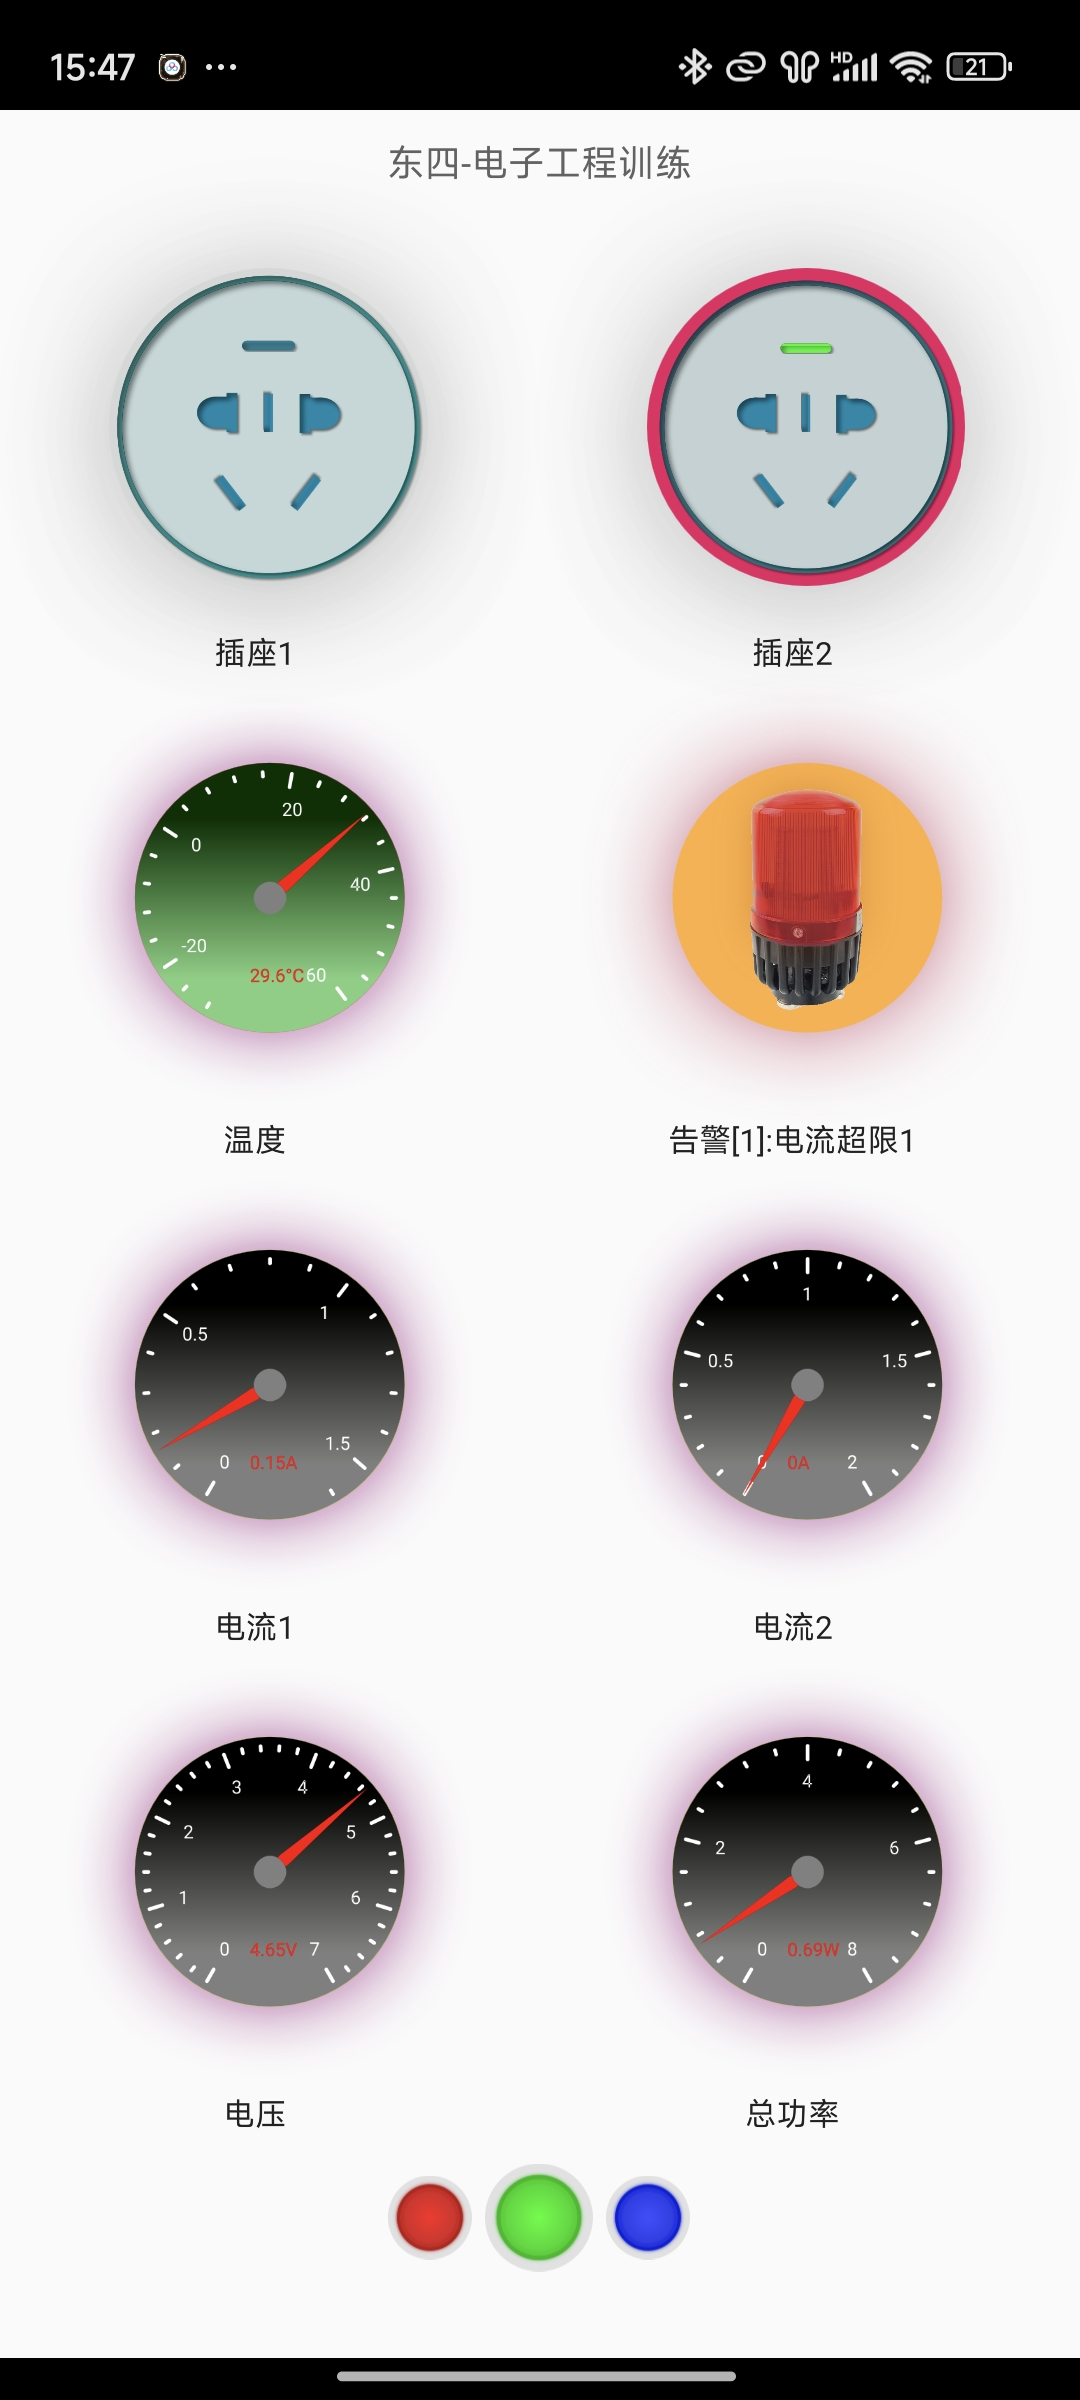
\includegraphics[width=.3\textwidth]{./figures/插座/系统调试/电流超限.jpg}
        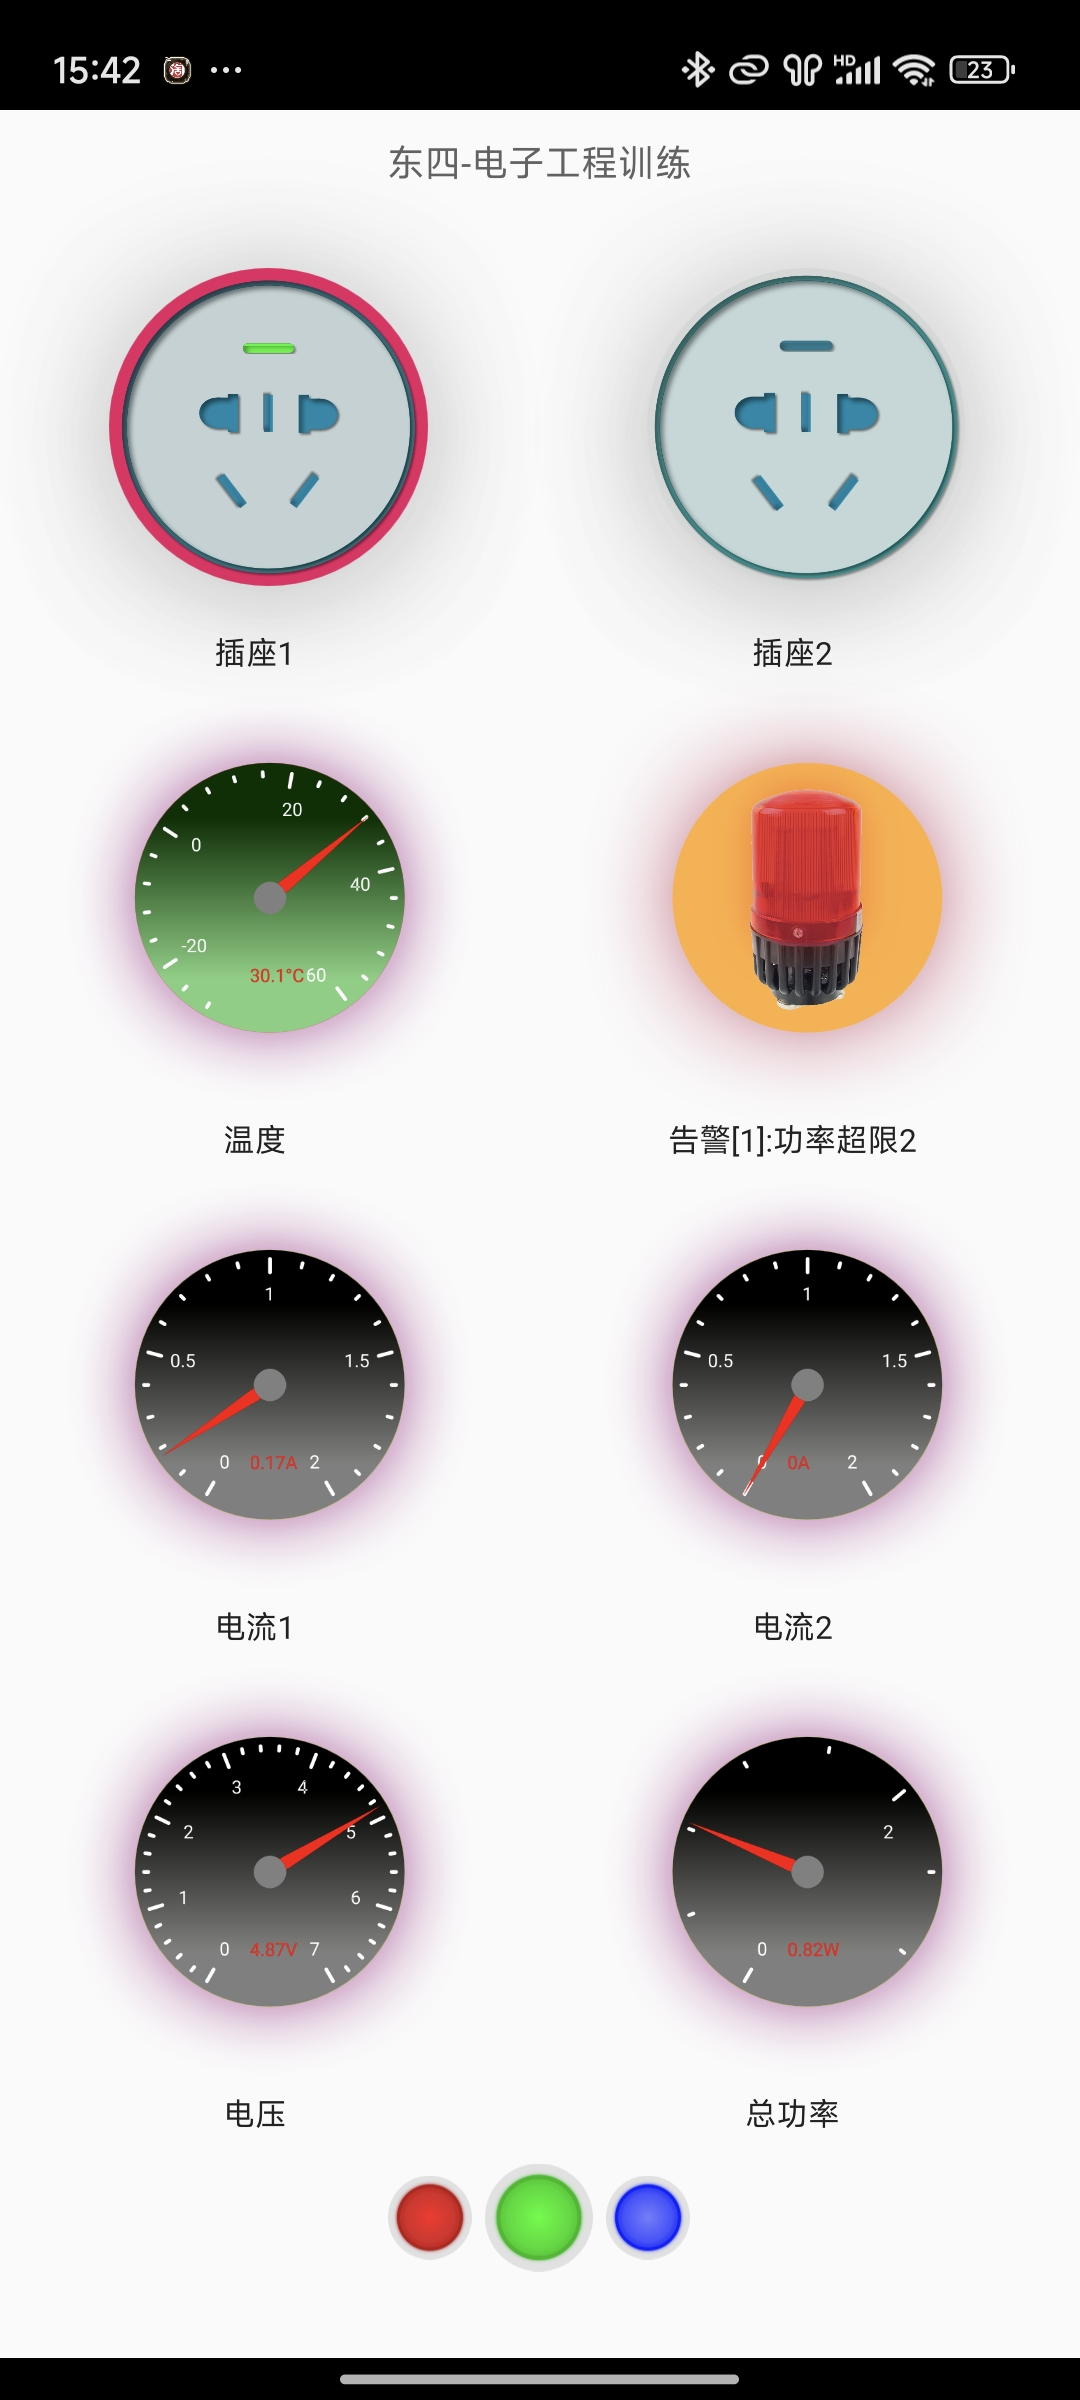
\includegraphics[width=.3\textwidth]{./figures/插座/系统调试/功率超限.jpg}
        \caption{插座关于电流和功率的告警}
        \label{电流}
      \end{figure}

    \item 测试子项目:超功率

    测试过程:设置功率上限为0.5W,接入小风扇并调至三档,立刻给出功率超限告警并断开了插座供电,如图(\ref{电流})所示。
    \item 测试子项目:温度告警

    测试过程:设置温度上限为31\textcelsius,下限设为最低,并用手加热温度传感器,当测量温度值超过设定温度上限时,app给出告警。
    待传感器恢复后将温度上限设为最高值,温度下限设为28\textcelsius,用风扇持续为温度传感器降温,待读数低于设定值时,app同样给出告警,并断开了插座供电,如图(\ref{温度})所示。

    \begin{figure}[htbp]
        \centering
        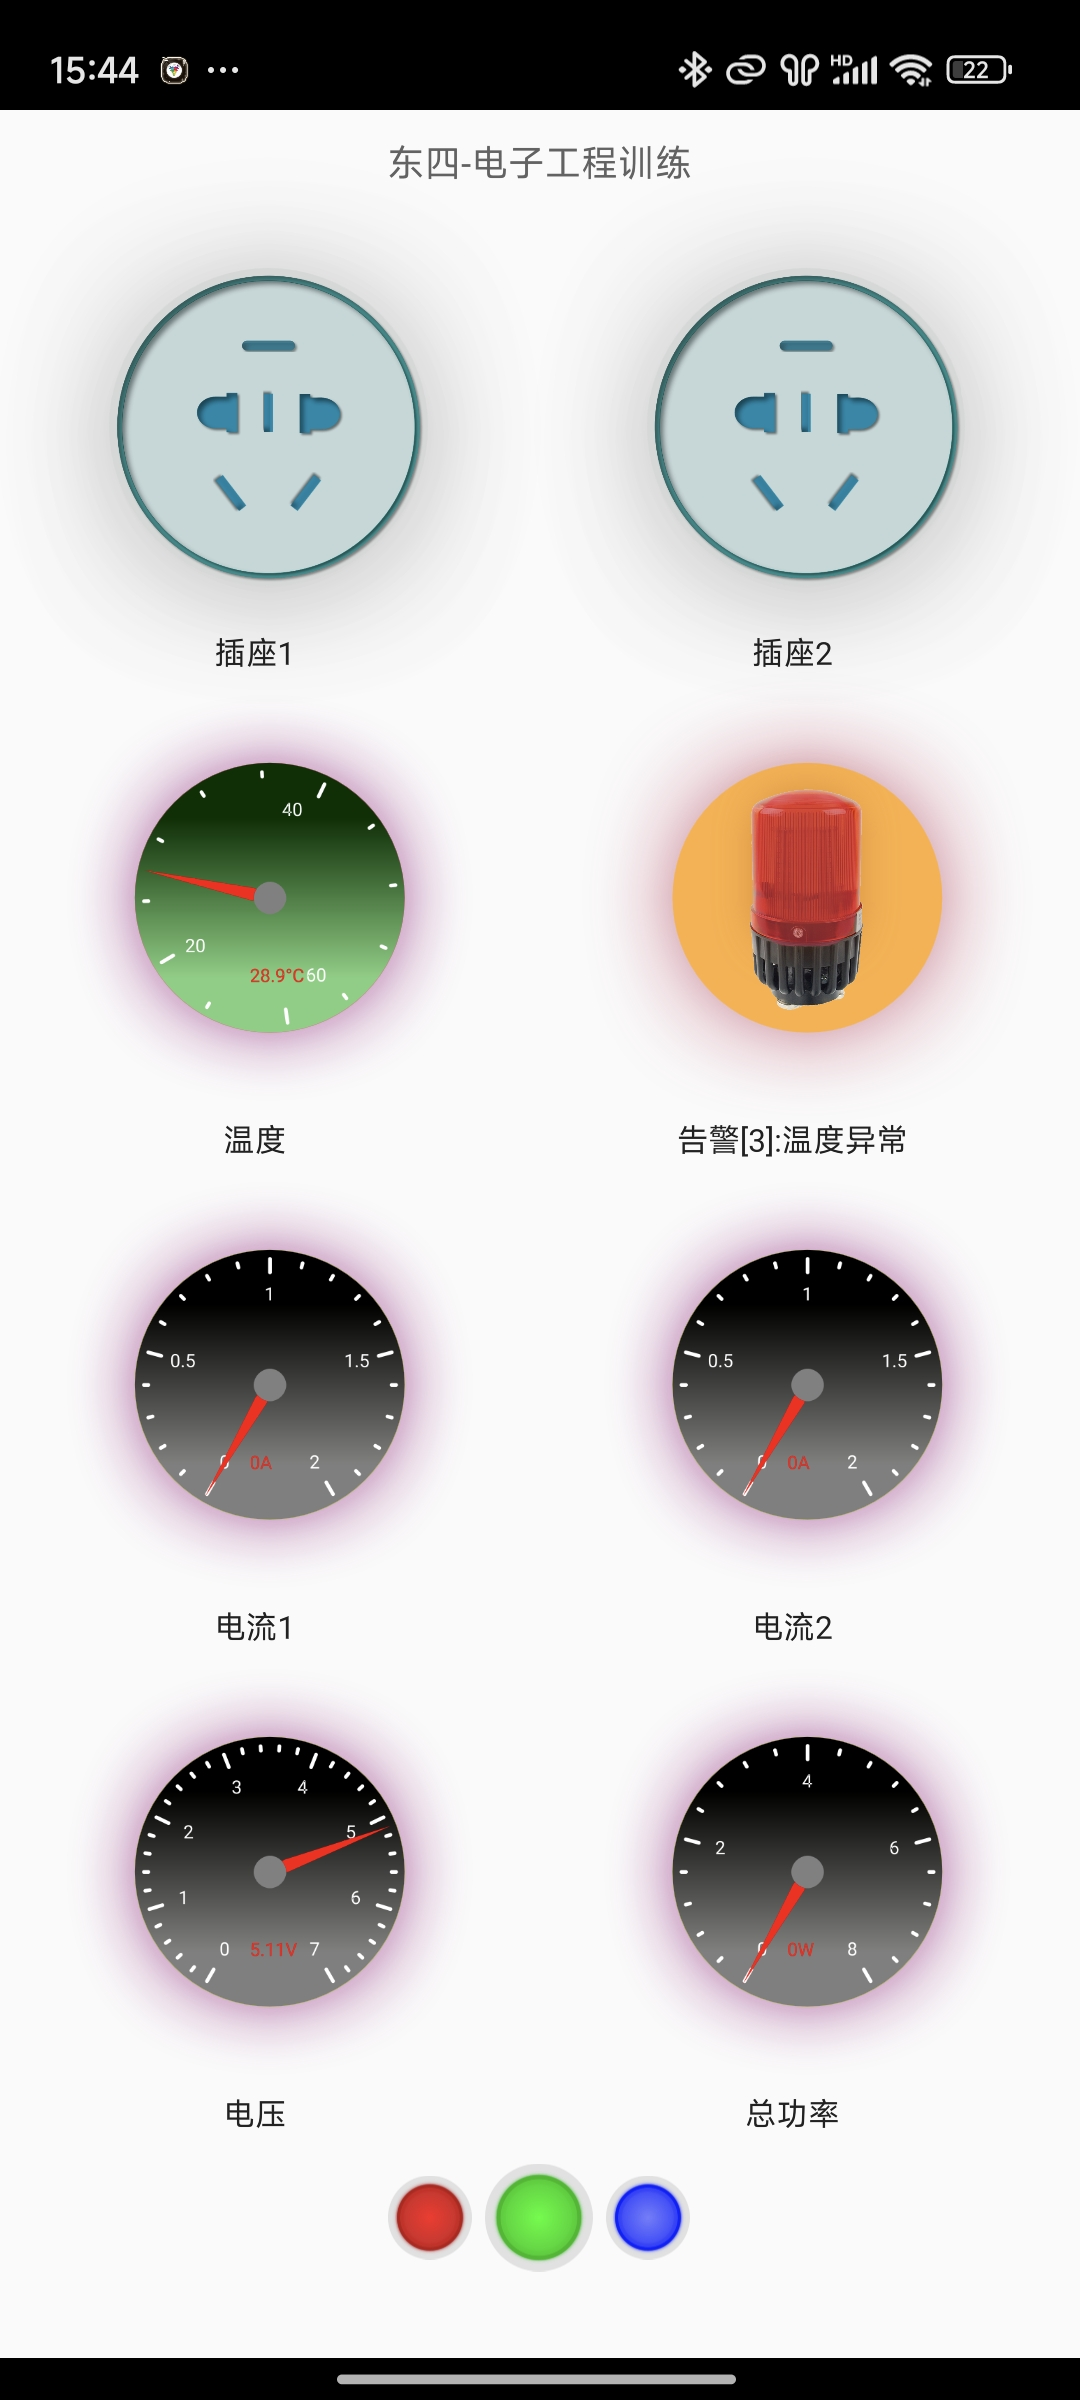
\includegraphics[width=.3\textwidth]{./figures/插座/系统调试/温度过低.jpg}
        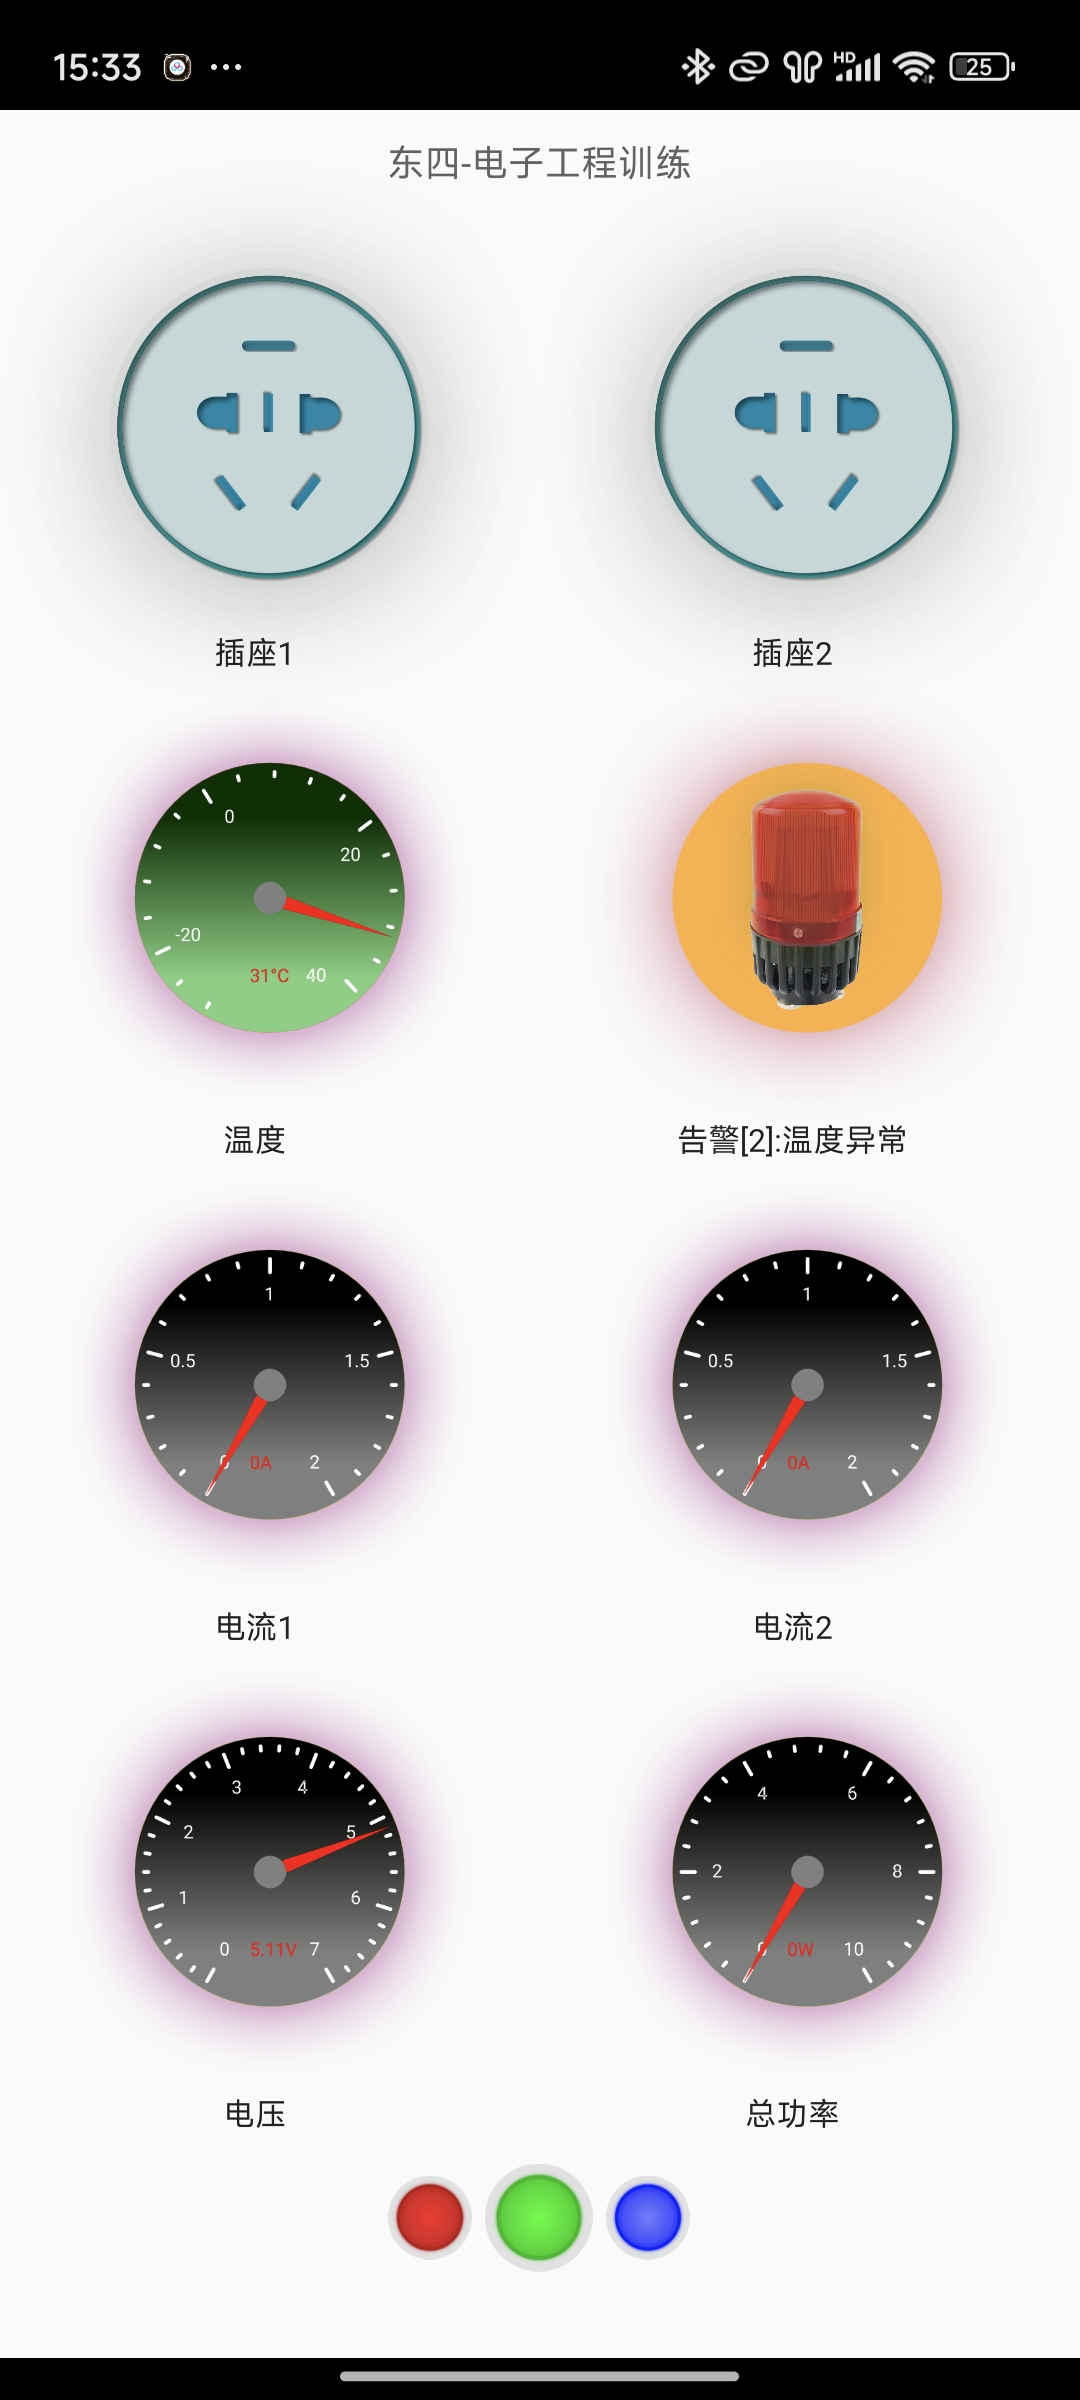
\includegraphics[width=.3\textwidth]{./figures/插座/系统调试/温度过高.jpg}
        \caption{插座关于温度的告警}
        \label{温度}
      \end{figure}
  \end{enumerate}
\end{enumerate}